\section{Polygonal Meshes}
\label{sec:polygonal}

In this section, we introduce polygonal meshes, describe a data structure to efficiently
work with them, and define the Euler characteristic.

\subsection{What is a surface?}

 Many surfaces are made up of many vertices, edges, and
triangles (or other polygons). We call such a surface a \emph{mesh}
or triangulated mesh, if all faces are triangles.
An example of a triangular mesh is shown in \figref{cat}.


 \begin{figure}[htb]
         \centering
        \begin{subfigure}[b]{0.3\textwidth}
         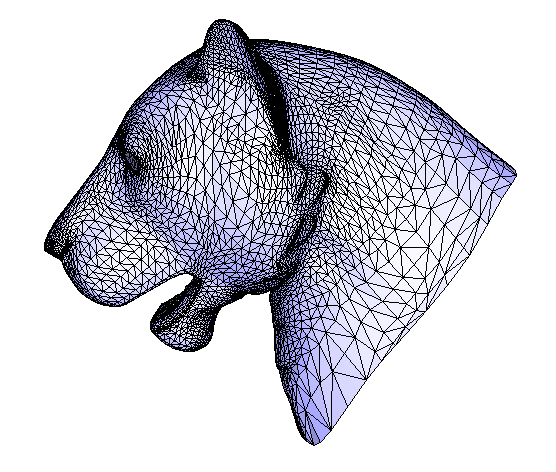
\includegraphics[width=\textwidth]{polygonal-mesh/profile}
         \caption{}
 	 \label{fig:profile}
       \end{subfigure}
         \hspace{.6cm}
         \begin{subfigure}[b]{0.19\textwidth}
         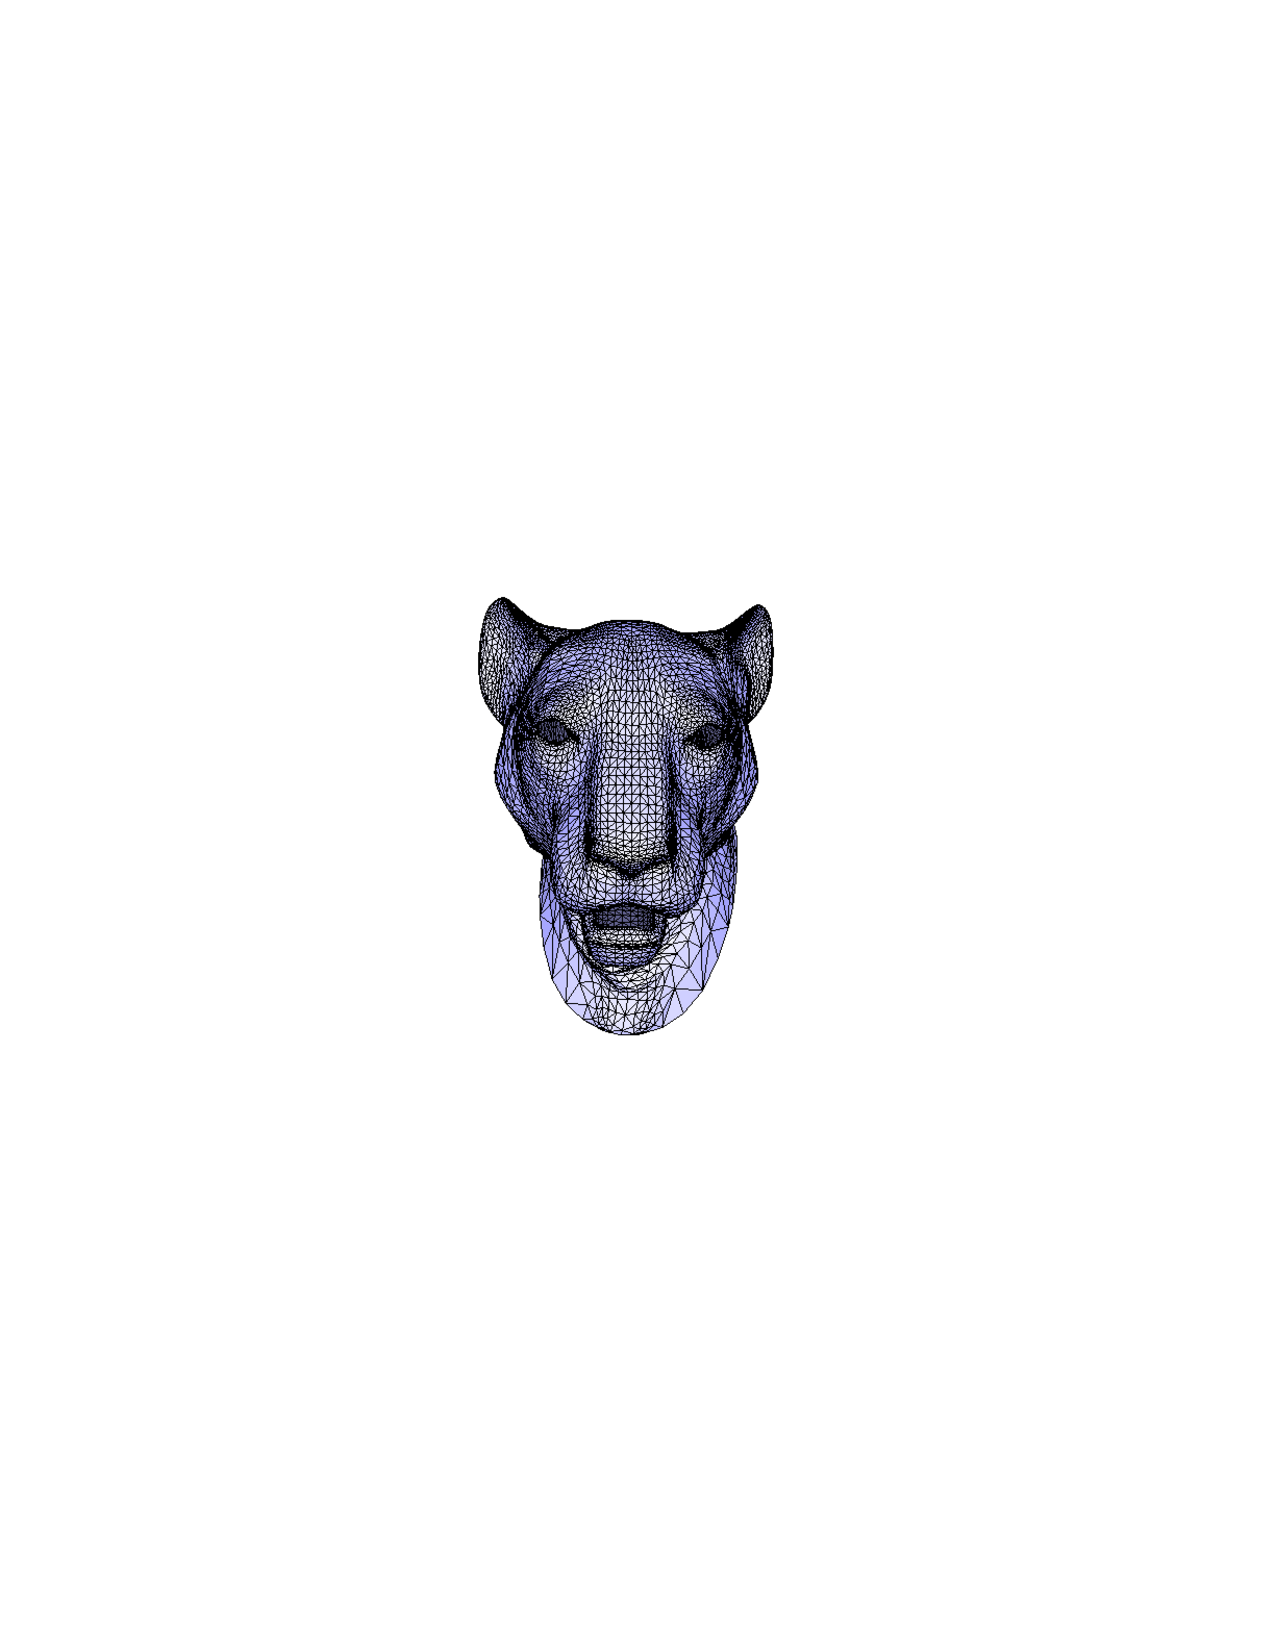
\includegraphics[width=\textwidth]{polygonal-mesh/head-on}
         \caption{}
          \label{fig:head-on}
         \end{subfigure}
             \hspace{.6cm}
         \begin{subfigure}[b]{0.24\textwidth}
         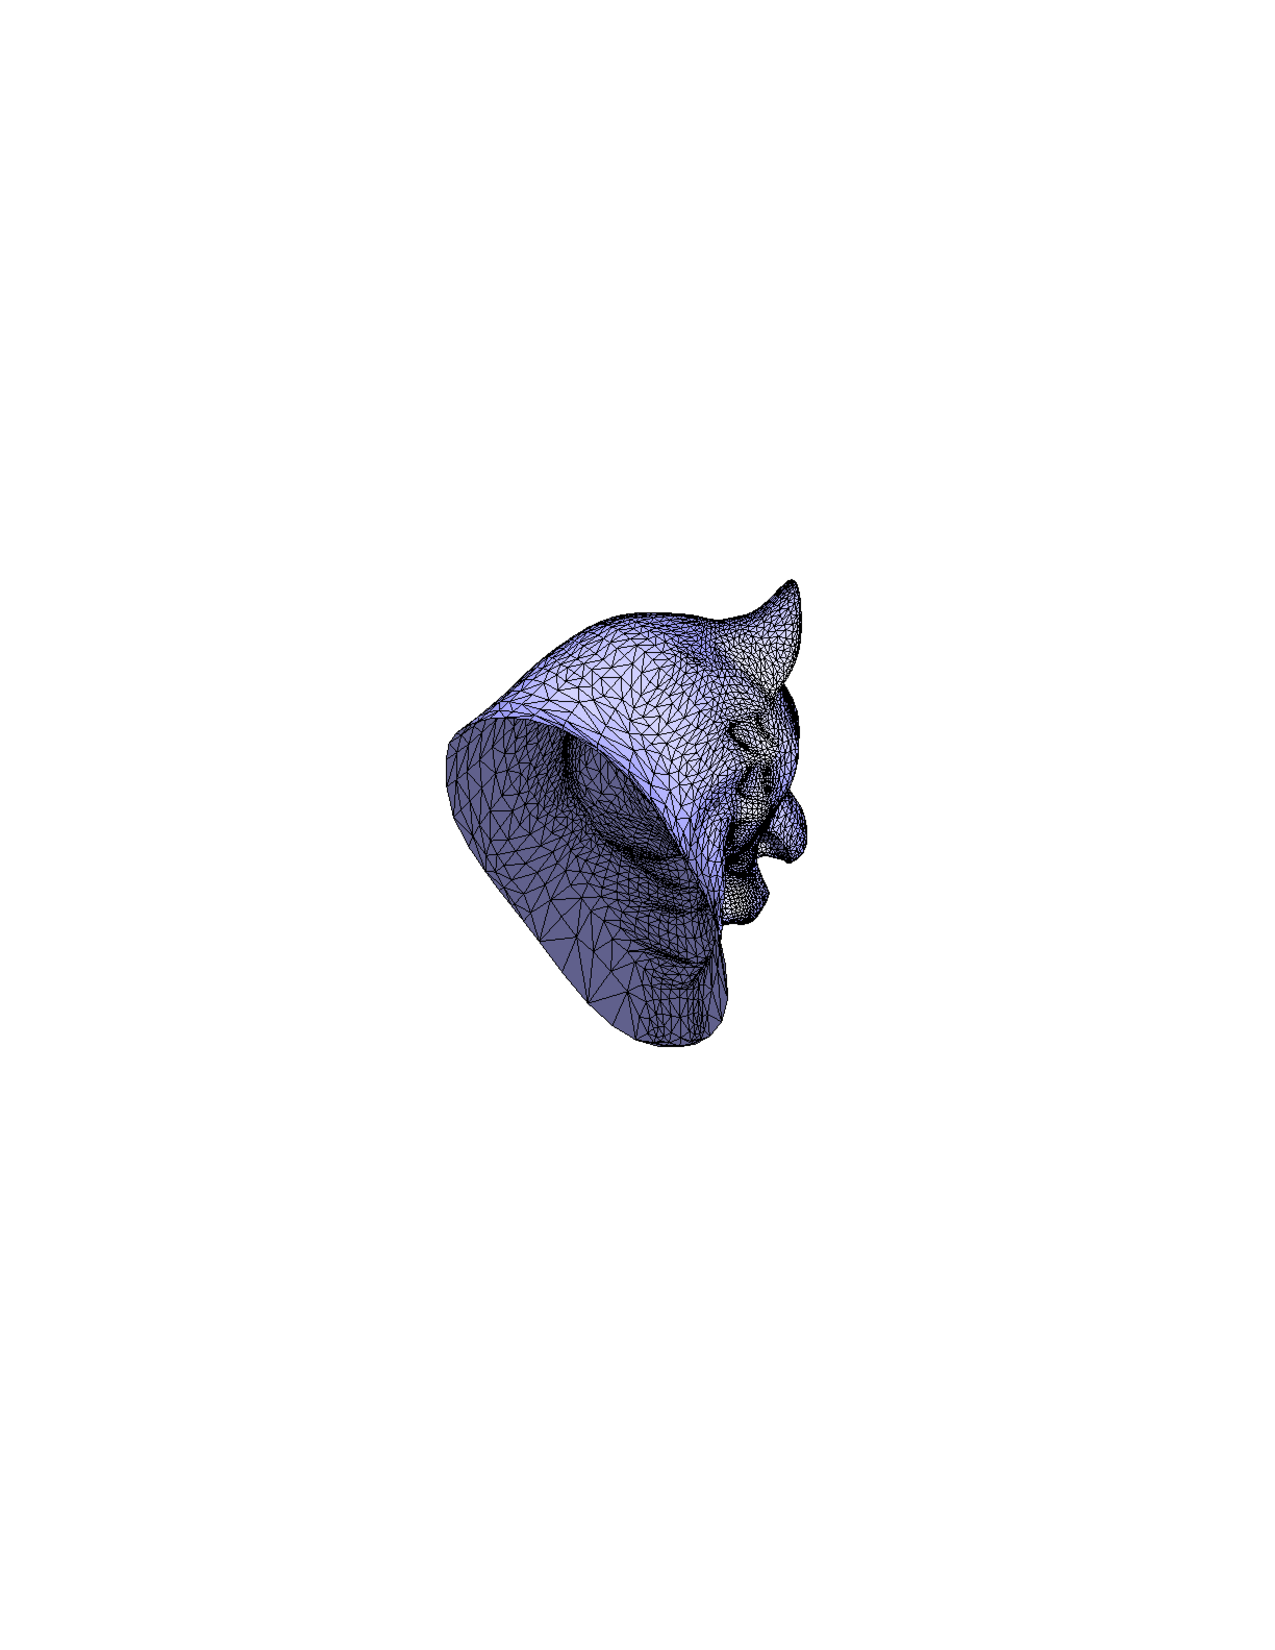
\includegraphics[width=\textwidth]{polygonal-mesh/back}
         \caption{}
          \label{fig:back}
         \end{subfigure}
		\caption{(\subref{fig:profile}) A profile view of a mesh.
 		(\subref{fig:head-on})  A head on view of the same mesh and the view from the back (\subref{fig:back}).
 		\label{fig:cat}}
 \end{figure}

One way to store a mesh in a computer is as a OFF file.
The first optional line of an OFF file identifies the file as an OFF file.
The second line lists the number of vertices, faces, and edges.
A list of vertices in $(x,y,z)$ coordinates is then given followed
by a list of faces indicated by the index of the vertices contained in the face.
For the mesh in \figref{cat}, the OFF file looks is shown in 
\tabref{off}.

\begin{table}[h!]
\caption{The OFF data for the mesh in \figref{cat}.}
\centering
\begin{tabular}{|p{2cm} p{2cm} p{2cm} p{2cm}|} 
 \hline
\texttt{OFF} &  & &  \\ 
\texttt{7529} & \texttt{14859} & \texttt{0} &  \\ 
\texttt{-0.29196} & \texttt{-0.0867173} & \texttt{-0.355149}  &  \\
 \texttt{-0.123586}   & \texttt{-0.0127199} & \texttt{-0.385597} &  \\
\texttt{-0.138255}   & \texttt{-0.0985078} & \texttt{-0.384018} &  \\
  & &\vdots &  \\  
 \texttt{3}&  \texttt{97} &\texttt{1893}& \texttt{1895}\\
 \texttt{3}& \texttt{71} & \texttt{1894} & \texttt{1893} \\
 \texttt{3} & \texttt{16} & \texttt{1895} & \texttt{1894}\\
   & &\vdots &  \\  
 \hline
\end{tabular}

\label{tab:off}
\end{table}

Suppose we work in a machine shop and a customer has an metal object that they would like
to duplicate.
One way to do this, is by 3D scanning the object to capture the coordinates on the 
surface and represent the object as a triangulated mesh, then use a machine to carve the object
from a block of metal. 
While scanning, errors might occur. As a result of these errors
we might obtain a triangulation that intersects itself. If we try to reconstruct the object
from our mesh our machines will have ambiguous information of what the surface of the object
should be.
This motivates developing an algorithm to determine if a mesh has self-intersections.


\noindent \textbf{Exercises}


\begin{enumerate}
	\item 
	
\end{enumerate}

\pagebreak